%
%\begin{center}
%\Large\textbf{\textsf{Exosquelette lombaire JAPET}}
%\normalsize
%\end{center}

%
%\ifprof
%\else
%\fi
%
%\ifprof
%\begin{corrige}
%\end{corrige}
%\else
%\fi
%
%
%\begin{figure}[!h]
%\centering
%\includegraphics[width=\textwidth]{}
%\caption{\label{ccs_mp_2023_fig_}  }
%\end{figure}
%




\section{Introduction}
\subsection{Présentation générale} %IA
\ifprof
\else
Les exosquelettes sont des solutions biomécaniques destinées à apporter une assistance ou un soutien physique à ceux qui les utilisent. La figure \ref{ccs_mp_2023_fig_01} représente l'exosquelette lombaire conçu par la société Japet. Il se présente sous la forme de deux ceintures (basse et haute) reliées par quatre actionneurs linéaires qui accompagnent les mouvements du patient tout en permettant un soutien de la colonne vertébrale.
\
%\begin{figure}[h]
%\begin{center}
%\captionsetup{labelformat=empty}
%\caption{bouton de réglage de la précontrainte}
%  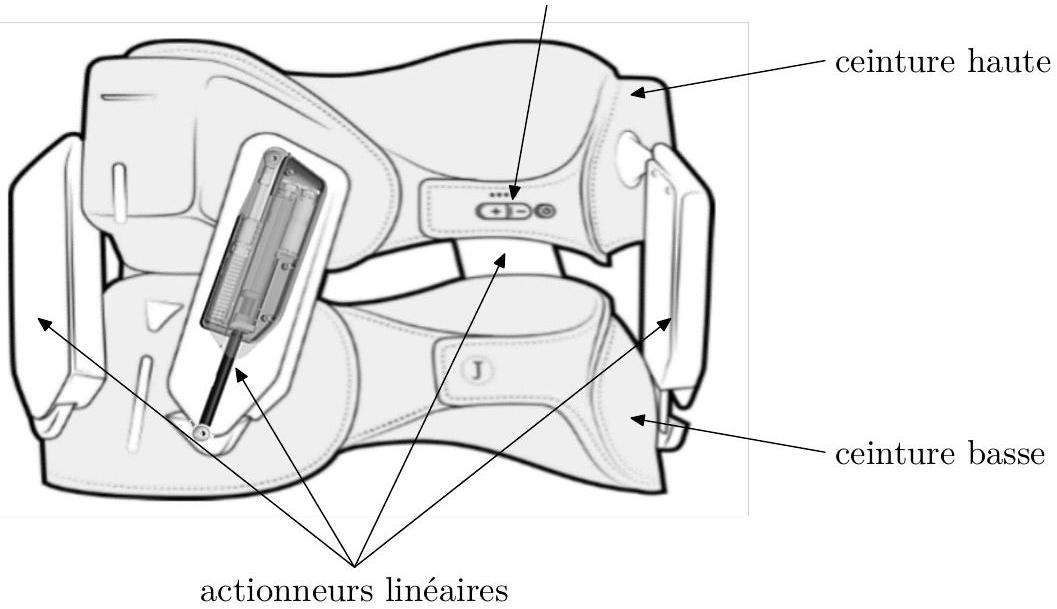
\includegraphics[width=\textwidth]{2025_09_16_5f2d7643f7e649c6833dg-01}
%\end{center}
%\end{figure}
%Figure 1 Exosquelette lombaire Japet



\begin{figure}[!h]
\centering
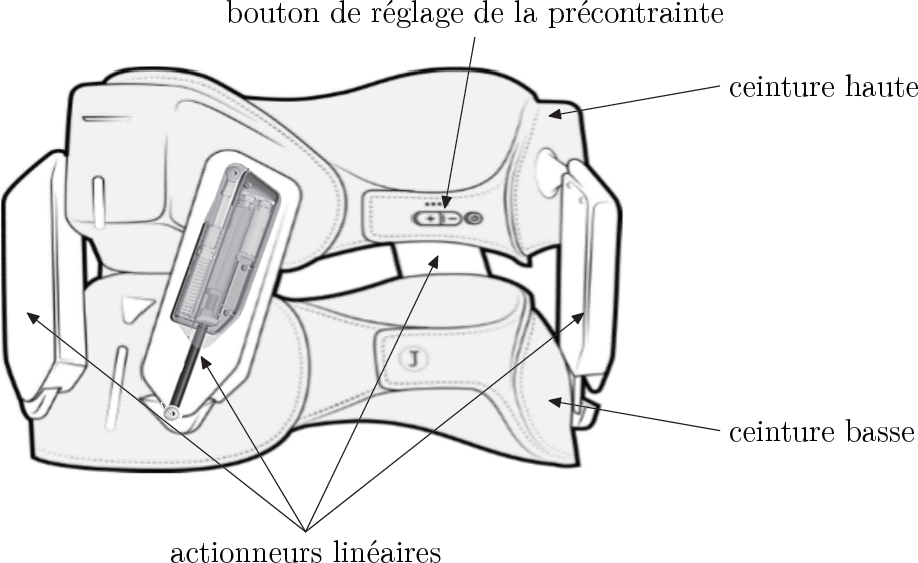
\includegraphics[width=.5\textwidth]{2023_mp_ccs_fig_01}
\caption{\label{ccs_mp_2023_fig_01}  Exosquelette lombaire Japet}
\end{figure}


Cet exosquelette lombaire est en priorité destiné au marché du travail et a vocation à soulager les salariés qui l'utilisent dans leurs mouvements quotidiens, en particulier dans les domaines de l'industrie ou de la logistique. Il est également destiné au soin de patients souffrant de lombalgie, en hôpital ou à domicile. Cet exosquelette n'a pas pour but d'augmenter les capacités physiques de l'être humain mais de les maintenir à un niveau satisfaisant. Cette assistance permet ainsi de conserver une activité professionnelle normale.

Grâce à l'effort de traction créé par les quatre actionneurs linéaires, le dispositif diminue la pression sur la colonne vertébrale afin de limiter la compression lombaire et soulager l'utilisateur des douleurs. Le système suit les mouvements de l'utilisateur en temps réel afin de conserver une liberté de mouvement totale et de préserver l'activité musculaire.
\fi
\subsection{Pré-dimensionnement des quatre actionneurs} %IB
\begin{obj}
Quantifier la force de traction à exercer par chaque actionneur linéaire pour atteindre un seuil de diminution de la pression intra-discale.
\end{obj}
\ifprof
\else

La société Japet a développé un modèle numérique biomécanique (figure \ref{ccs_mp_2023_fig_02} à gauche) du corps humain permettant de déterminer la valeur de la force de traction à exercer par les actionneurs pour soulager les disques intervertébraux en diminuant la pression intra-discale.\\
Le modèle numérique biomécanique a permis d'obtenir les courbes de la figure \ref{ccs_mp_2023_fig_03} décrivant les évolutions des pressions intra-discales entre les vertèbres L3-L4 et L4-L5. Celles-ci ont été obtenues dans les conditions de simulation suivantes :

\begin{itemize}
  \item colonne vertébrale verticale ;
  \item chaque actionneur linéaire développe une force de traction progressivement de 0 à \SI{100}{N} ;
  \item l'évolution des forces de traction est lente afin de négliger les effets dynamiques.
\end{itemize}
\fi

%Q 1. \ref{ccs_mp_2023_q_}
\question{\label{ccs_mp_2023_q_01}
Après analyse des courbes de la figure \ref{ccs_mp_2023_fig_03}, justifier que la force de traction choisie par le constructeur, afin de limiter la pression intra-discale, est de 40 N par actionneur.}
\ifprof
\begin{corrige}
On constate à la lecture des courbes qu'au-delà de \SI{40}{N} de traction des vérins, la pression discale n'est plus diminuée. C'est surement la raison qui a poussé le constructeur à limiter l'effort de traction à \SI{40}{N}.
\end{corrige}
\else
\fi

%\begin{figure}[h]
%\begin{center}
%  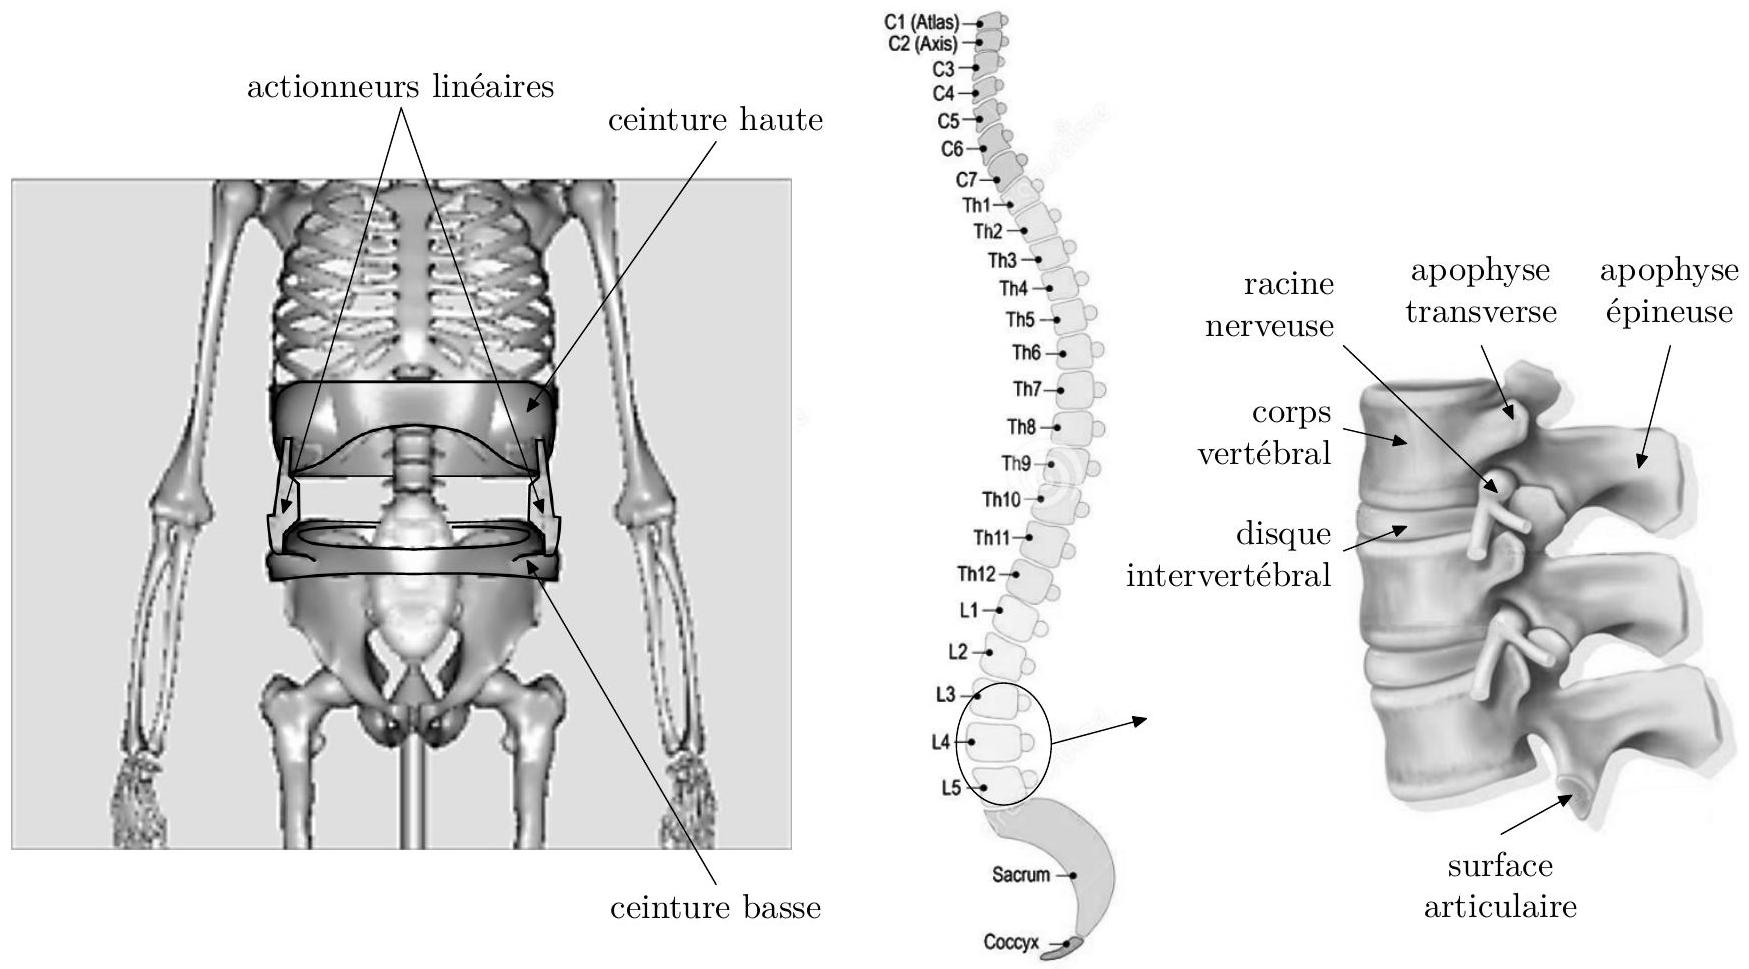
\includegraphics[width=\textwidth]{2025_09_16_5f2d7643f7e649c6833dg-02(1)}
%\captionsetup{labelformat=empty}
%\caption{Figure 2 Modèle numérique biomécanique (à gauche) et détail de la structure vertébrale avec numérotation des vertèbres (à droite)}
%\end{center}
%\end{figure}

\ifprof
\else

\begin{figure}[!h]
\centering
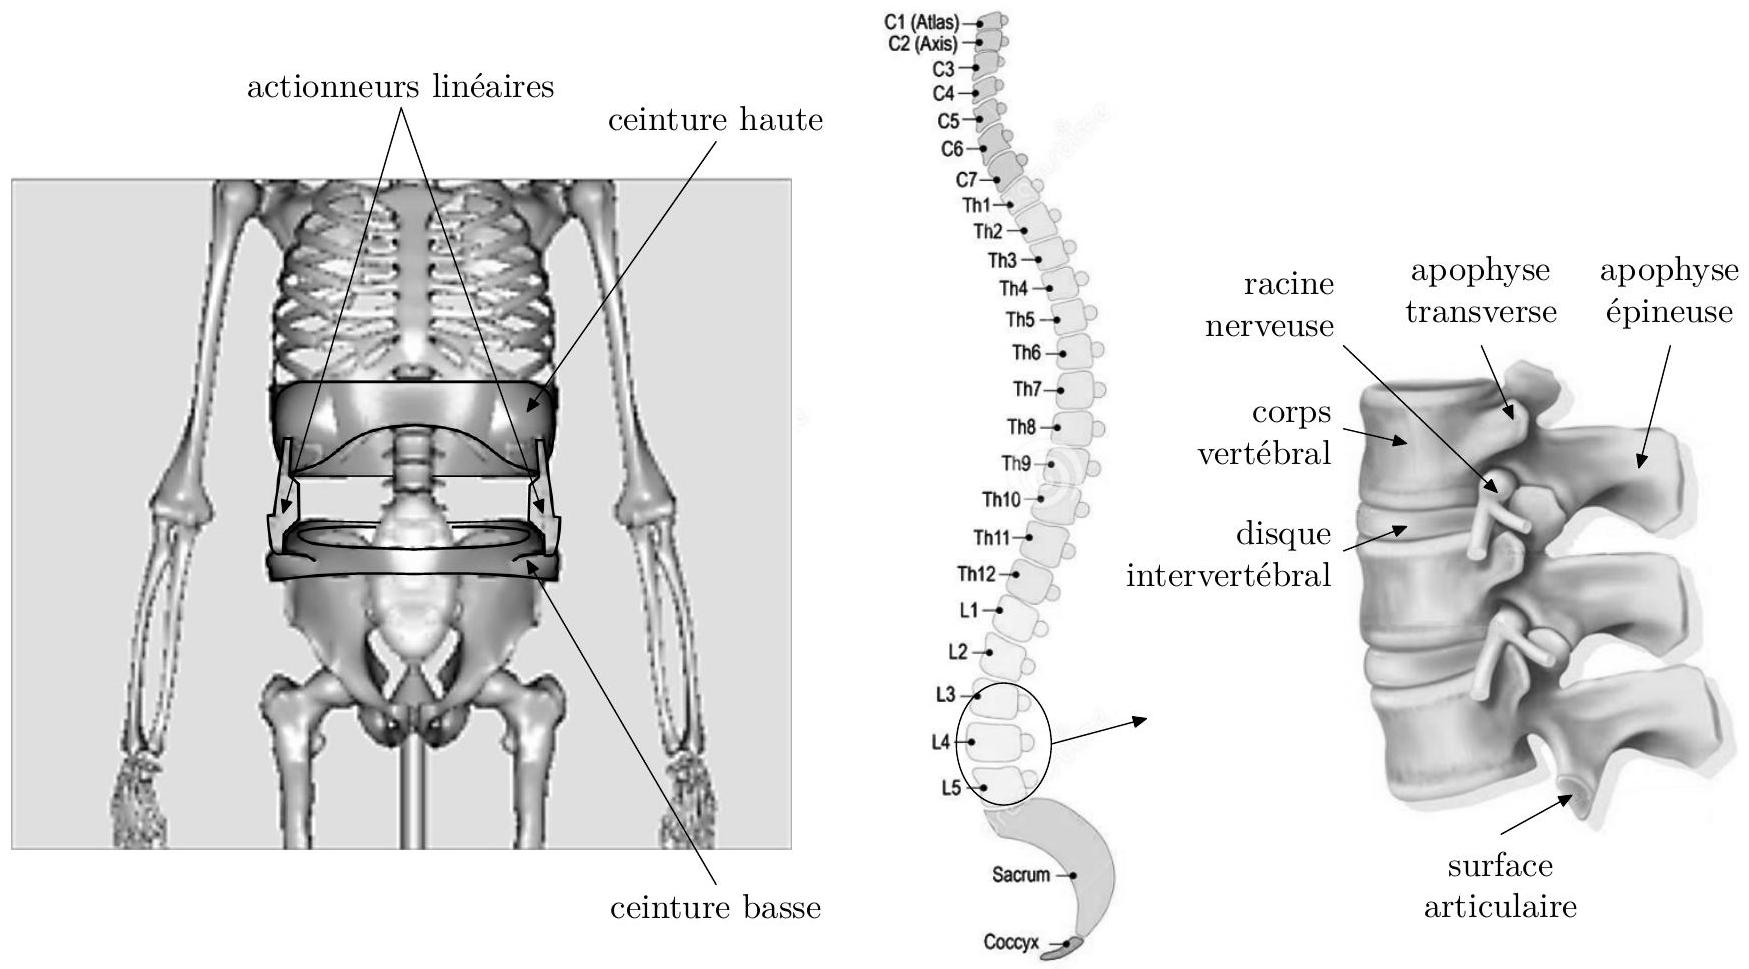
\includegraphics[width=\textwidth]{2025_09_16_5f2d7643f7e649c6833dg-02(1)}
\caption{\label{ccs_mp_2023_fig_02}  Modèle numérique biomécanique (à gauche) et détail de la structure vertébrale avec numérotation des vertèbres (à droite)}
\end{figure}

\fi


%
%\begin{figure}[h]
%\begin{center}
%  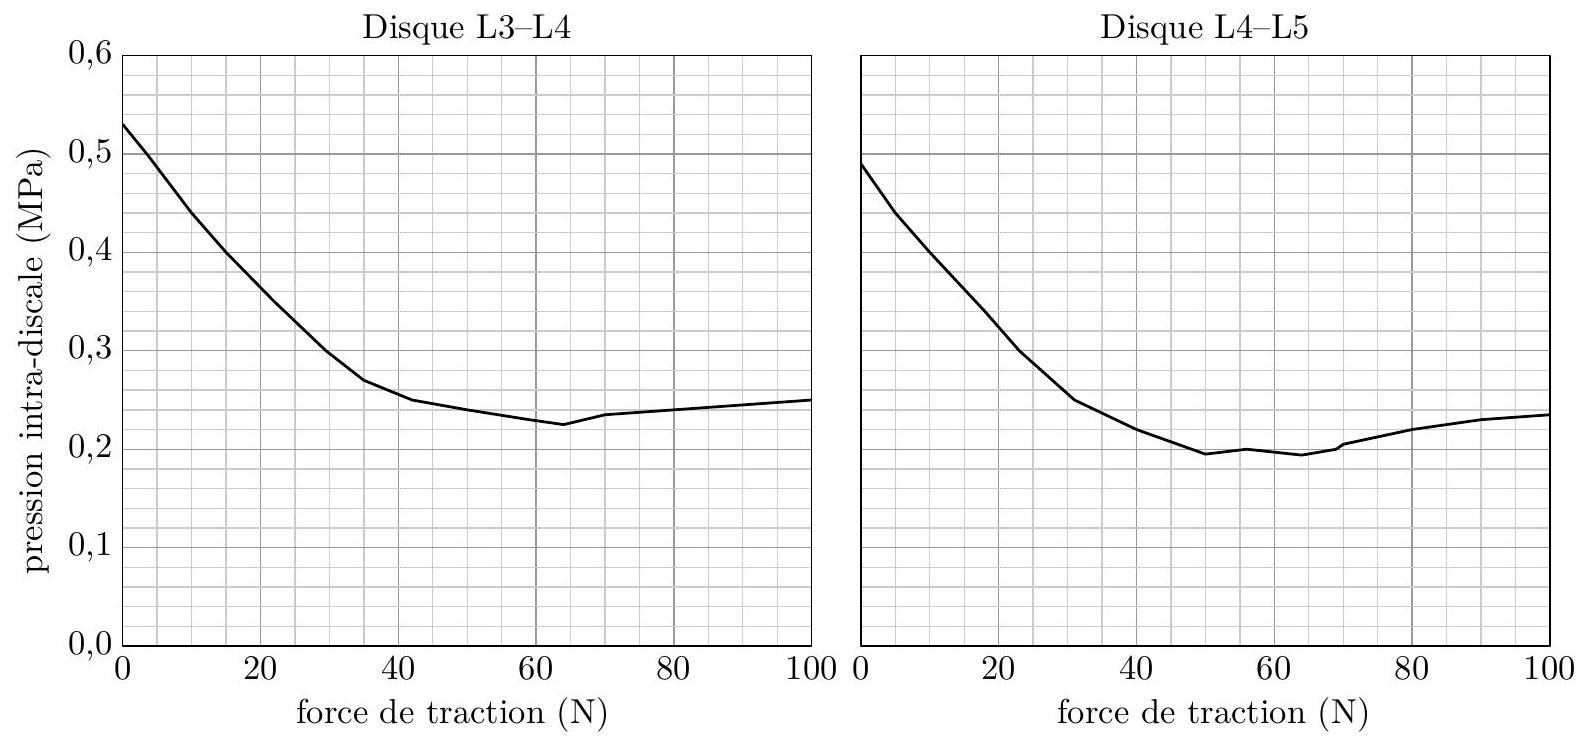
\includegraphics[width=\textwidth]{2025_09_16_5f2d7643f7e649c6833dg-02}
%\captionsetup{labelformat=empty}
%\caption{Figure 3 Évolution de la pression intra-discale simulée en L3-L4 et L4-L5 en fonction de la force de traction développée par un seul actionneur linéaire}
%\end{center}
%\end{figure}



\ifprof
\else

\begin{figure}[!h]
\centering
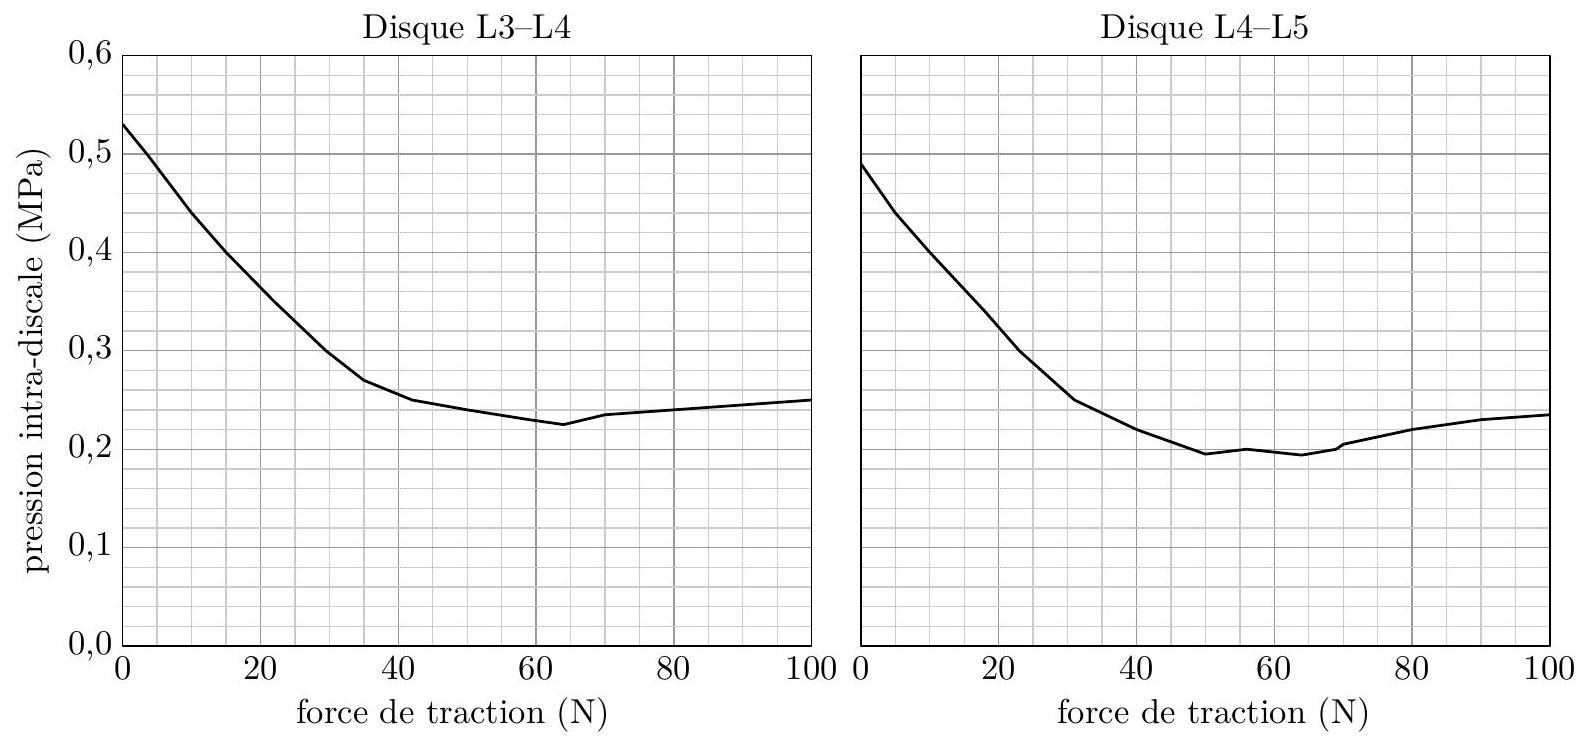
\includegraphics[width=\textwidth]{2025_09_16_5f2d7643f7e649c6833dg-02}
\caption{\label{ccs_mp_2023_fig_03}  Évolution de la pression intra-discale simulée en L3-L4 et L4-L5 en fonction de la force de traction développée par un seul actionneur linéaire}
\end{figure}

\fi


%IC
\subsection{Validation expérimentale du pré-dimensionnement des quatre actionneurs linéaires}
\begin{obj}
%Objectif\\
Montrer qu'il est possible de diminuer la pression intra-discale de 25 à $50 \%$ dans le cas d'une utilisation au quotidien de l'exosquelette.
\end{obj}
\ifprof
\else


Des capteurs de pression ont été positionnés sur un cadavre (équipé de l'exosquelette Japet) dans le disque intervertébral L3-L4 en trois positions différentes du disque (avant, milieu, arrière) afin de mesurer la pression intra-discale réelle. Un effort de traction a été appliqué pour valider expérimentalement la baisse de pression intra-discale entre les vertèbres. Celles-ci ont été obtenues dans les conditions d'expérimentation suivantes :

\begin{itemize}
  \item à l'instant $t=0$, et pour une durée de 2 minutes, chaque actionneur linéaire développe une force de traction constante égale à \SI{40}{N} ;
  \item à l'instant $t=2 \mathrm{~min}$, les forces de traction sont annulées.
\end{itemize}

%\begin{figure}[h]
%\begin{center}
%  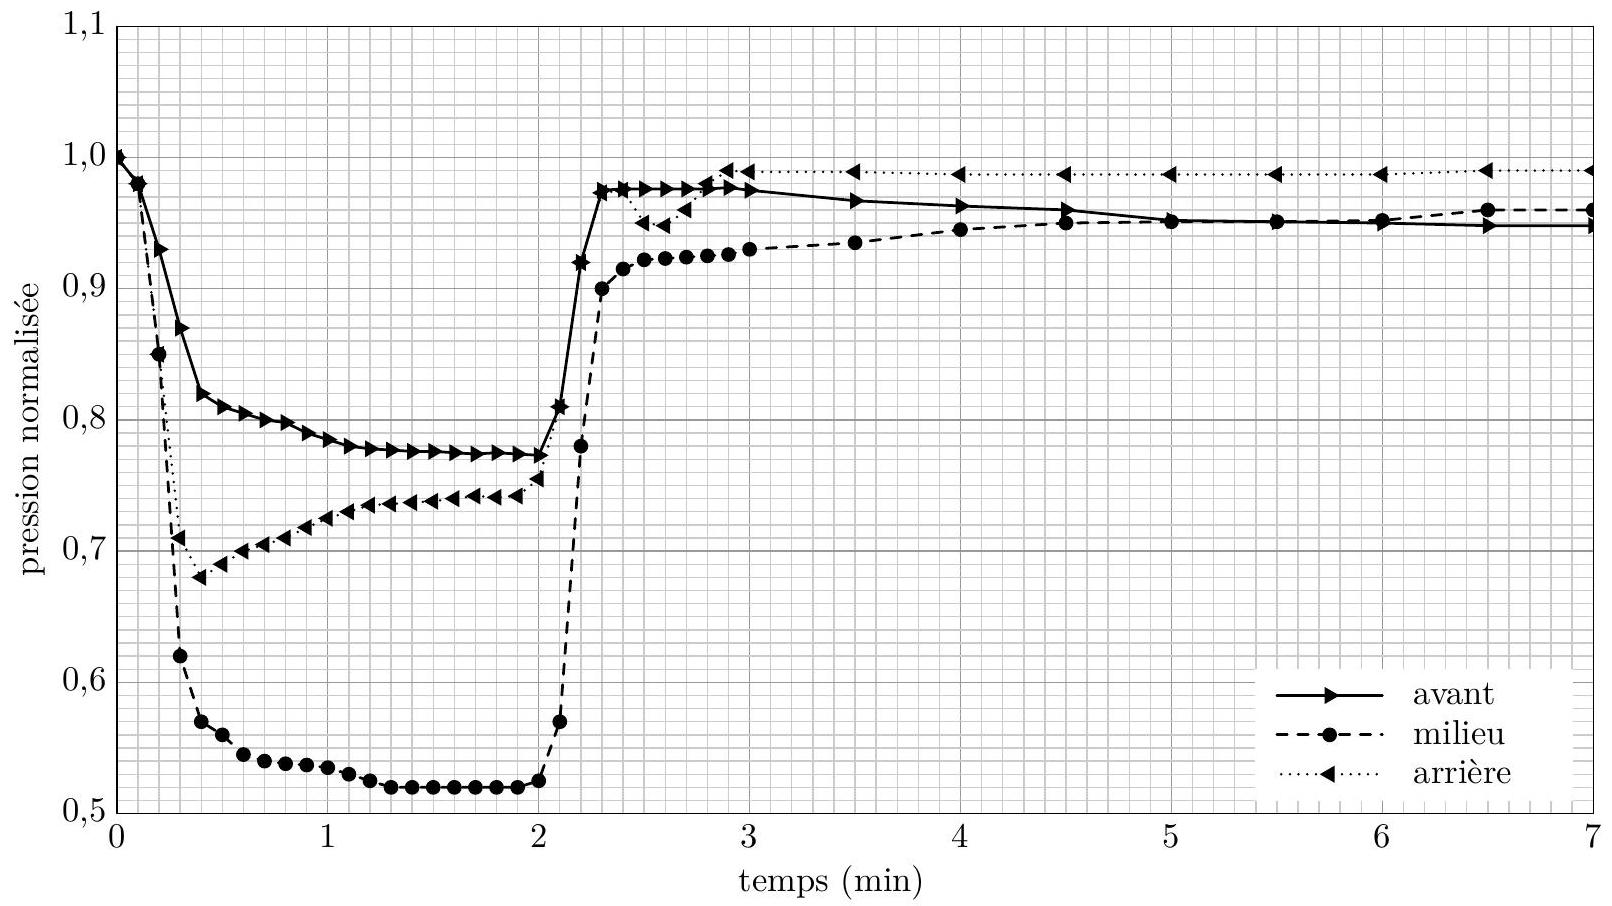
\includegraphics[width=\textwidth]{2025_09_16_5f2d7643f7e649c6833dg-03}
%\captionsetup{labelformat=empty}
%\caption{Figure 4 Évolution de la pression intra-discale mesurée et normalisée dans les trois positions du disque intervertébral L3-L4}
%\end{center}
%\end{figure}

\begin{figure}[!h]
\centering
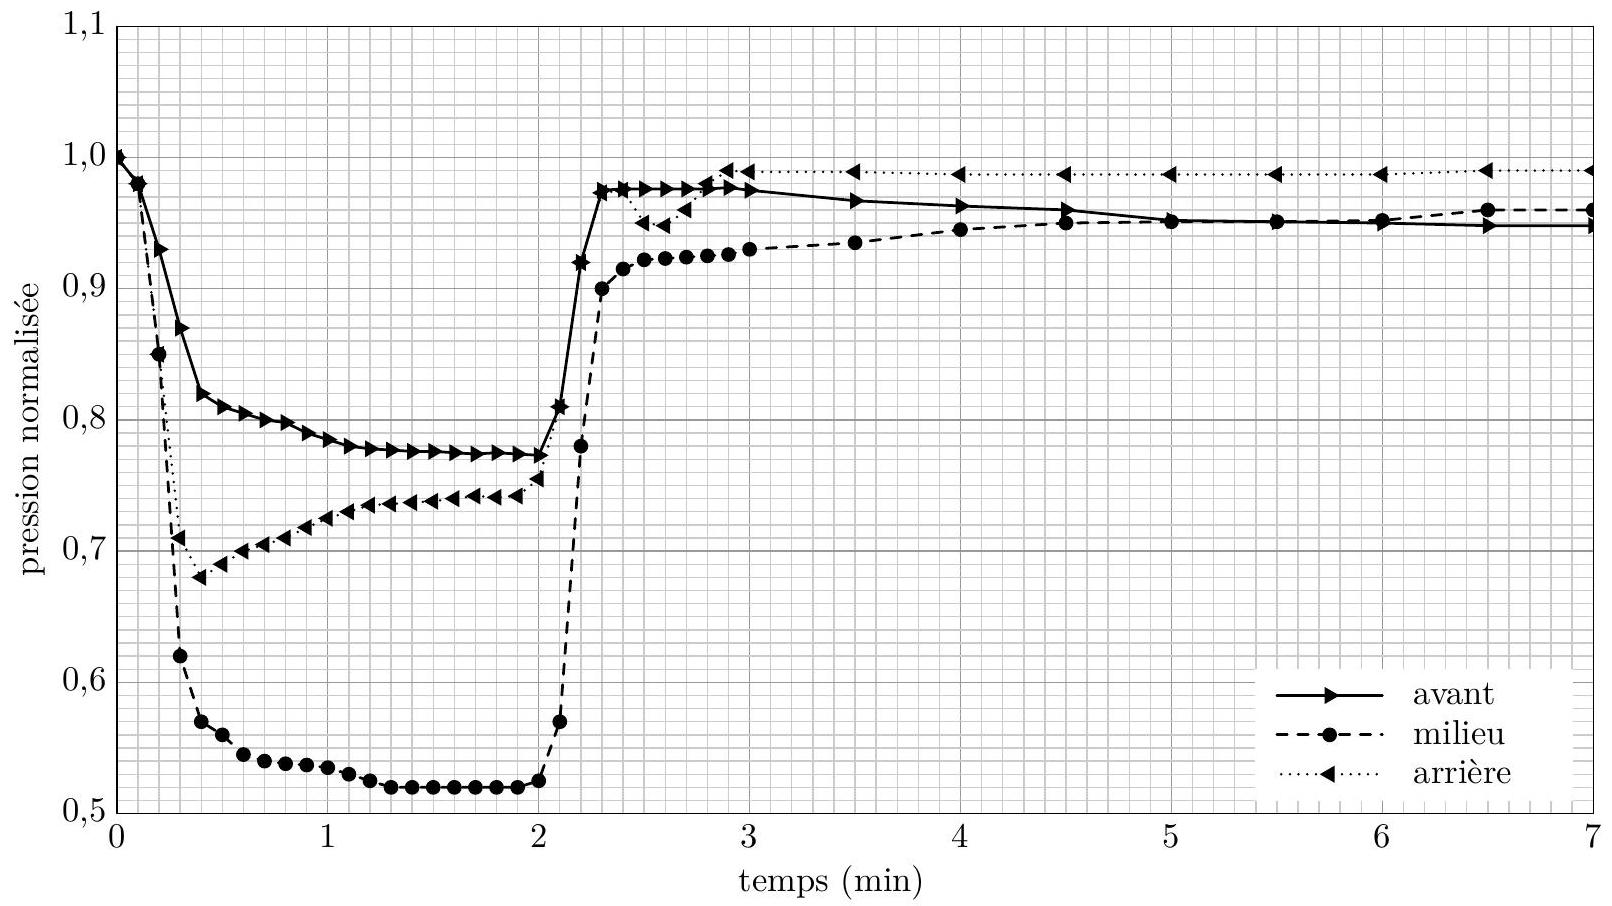
\includegraphics[width=\textwidth]{2025_09_16_5f2d7643f7e649c6833dg-03}
\caption{\label{ccs_mp_2023_fig_04}  Évolution de la pression intra-discale mesurée et normalisée dans les trois positions du disque intervertébral L3-L4}
\end{figure}



Les résultats ont été normalisés afin de tenir compte des conditions initiales ( $t<0$ ) en divisant les pressions mesurées par la pression intervertébrale initiale. Ils sont présentés sur la figure \ref{ccs_mp_2023_fig_04}.
\fi

\question{\label{ccs_mp_2023_q_02}
Déterminer, pour les trois positions du capteur de pression dans le disque intervertébral L3-L4, la diminution moyenne de la pression intra-discale (en \%) pendant les deux minutes d'application de l'effort de traction, sans prendre en compte la phase transitoire de 0 à $0,5 \mathrm{~min}$.}
\ifprof
\begin{corrige}
\begin{itemize}
\item Capteur en position avant : en régime permanent, la pression normalisée est de 0,78 soit une diminution de la pression de 22\; \%.
\item Capteur en position arrière : en régime permanent, la pression normalisée est de 0,74 soit une diminution de la pression de 24\; \%.
\item Capteur en position milieu : en régime permanent, la pression normalisée est de 0,52 soit une diminution de la pression de 48; \%.
\end{itemize}
Les vérins diminuent globalement la pression interdiscale, notamment sur la partie centrale du disque.
\end{corrige}
\else
\fi

\ifprof
\else

Cette pré-étude théorique ainsi que la validation expérimentale permettent de montrer l'efficacité du soulagement intra-discal par un système externe actif. Le développement de l'exosquelette est basé sur ces résultats. L'analyse des résultats des expérimentations décrites précédemment a permis de définir le cahier des charges partiel proposé dans le tableau \ref{ccs_mp_2023_tab_01}.

\begin{table}[h]
\begin{center}
\begin{tabular}{lp{5cm}p{5cm}ll}
\hline
\textbf{Id} & \textbf{Exigence} & \textbf{Critère} & \textbf{Niveau} & \textbf{Flexibilité} \\
\hline
\multirow[t]{2}{*}{Id1} & \multirow[t]{2}{4cm}{Limiter la compression lombaire pour soulager les douleurs} & Force de traction pour chaque actionneur linéaire & 40 N & $< \pm 2,5 \%$ \\
 &  & Vitesse maximale de la montée de la force de traction & $100 \mathrm{~N} \cdot \mathrm{~s}^{-1}$ & nulle \\
\hline
Id2 & Préserver l'activité musculaire, en garantissant la liberté de mouvement naturel du corps humain & Liberté totale de mouvement entre les ceintures basse et haute & 6 degrés de liberté & aucune \\
\hline
\end{tabular}
%\captionsetup{labelformat=empty}
\caption{Extrait du cahier des charges fonctionnel de l'exosquelette \label{ccs_mp_2023_tab_01}}
\end{center}
\end{table}
\fi

%I.D - 
\subsection{Problématique et organisation de l'étude}

\ifprof
\else

L'exosquelette lombaire, répertorié comme un système médical par les autorités de santé, doit garantir un fonctionnement sûr afin de ne causer aucun dommage à la colonne vertébrale tout en assurant une traction au niveau des vertèbres pour soulager les disques intervertébraux. Le mouvement naturel du corps devra être conservé. Ceci implique que l'amplitude des mouvements de l'exosquelette lombaire devra s'adapter aux mouvements du corps et que l'effort d'assistance devra correspondre aux valeurs définies dans le cahier des charges partiel.

La problématique globale du sujet est de valider un modèle de connaissance simulant la capacité des actionneurs linéaires à exercer un effort de traction maitrisé tout en garantissant la liberté de mouvement naturel du corps humain.\\
L'étude est limitée au mouvement de l'ensemble dans le plan sagittal (figure \ref{ccs_mp_2023_fig_05}). Pour aborder la problématique, l'étude s'intéresse à :

\begin{itemize}
  \item un degré de liberté particulier de la ceinture haute par rapport à la ceinture basse ;
  \item la capacité d'un actionneur linéaire à exercer une force de \SI{40}{N}.
\end{itemize}

%\begin{figure}[h]
%\begin{center}
%  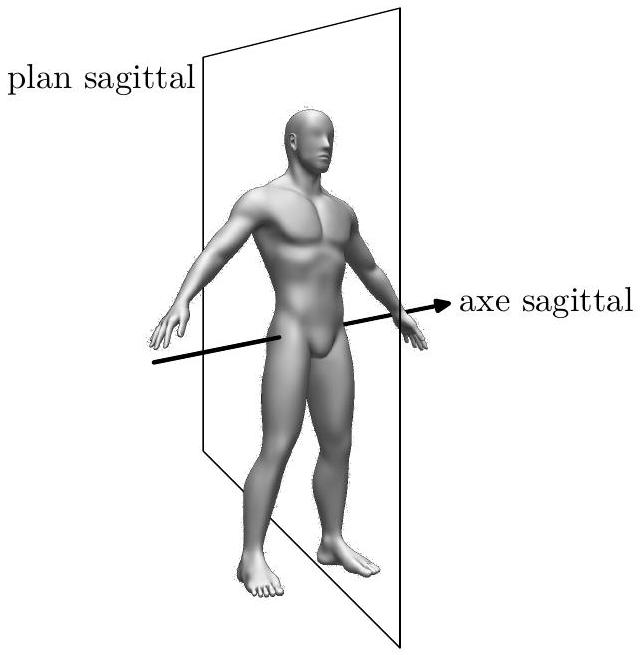
\includegraphics[width=\textwidth]{2025_09_16_5f2d7643f7e649c6833dg-04}
%\captionsetup{labelformat=empty}
%\caption{Figure 5 Plan et axe sagittal}
%\end{center}
%\end{figure}

\begin{figure}[!h]
\centering
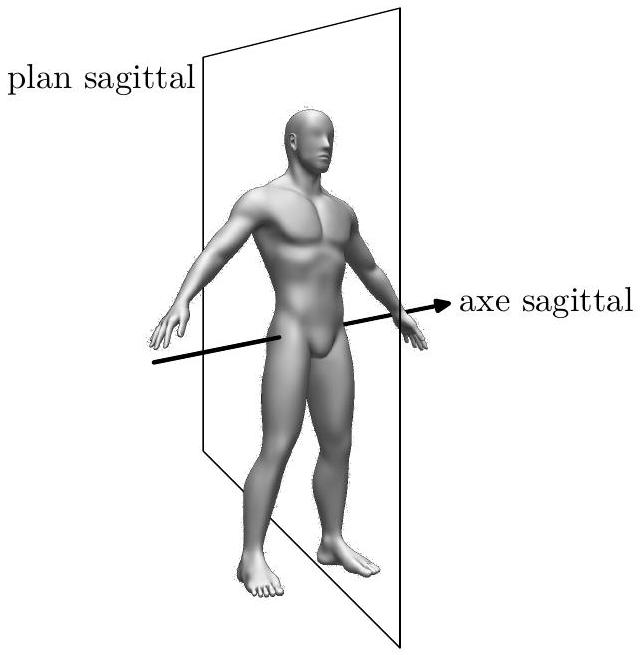
\includegraphics[width=.4\textwidth]{2025_09_16_5f2d7643f7e649c6833dg-04}
\caption{\label{ccs_mp_2023_fig_05}  Plan et axe sagittal}
\end{figure}


Après avoir déterminé l'amplitude nécessaire du déplacement des actionneurs linéaires, l'étude portera sur la caractérisation dynamique et la commande d'un des quatre actionneurs linéaires. Cette dernière nécessite l'élaboration d'un modèle de connaissance du système étudié. La société Japet a construit un banc d'essai et de mesure. Ce banc d'essai a pour finalité de :

\begin{itemize}
  \item contrôler l'amplitude nécessaire du déplacement des actionneurs linéaires ;
  \item comparer les résultats issus des simulations aux résultats expérimentaux pour une position particulière d'un actionneur linéaire, dans un premier temps.\\
Par la suite, le constructeur validera chaque actionneur linéaire commercialisé à l'aide du banc d'essai dans une démarche qualité.
\end{itemize}
\fi